\chapter{Determination of Substitutional Nitrogen Concentration via Fourier Infrared Transform Spectroscopy}
\label{chFTIRMethod}
\indent

This dissertation investigates specific substrate conditions and reactor parameters required to synthesize substrates optimized for laser writing. The ideal substrate must possess a sufficiently high concentration of substitutional nitrogen such that a substitutional nitrogen defect will exist within the focal volume of the laser while simultaneously minimizing nitrogen vacancy defects. Systematically evaluating the quality of grown films requires an accurate, non-destructive method for determining the concentration of substitutional nitrogen. A non-destructive method to quantify substitutional nitrogen in nitrogen-rich diamond was developed using FTIR. A recount of the development and validation of the non-destructive method is provided in this chapter.

\section{Shortcomings of Current Methods to Quantify Nitrogen Concentrations in Diamond}
\indent

As nitrogen is a common defect in diamond, there are several methods for characterizing nitrogen related defects. As is often the case, each method has strengths and weaknesses. A discussion of methods and their shortcomings is given in the following sections.

\subsection{Destructive Determination of Nitrogen via Secondary Ion Mass Spectrometry}
\indent

Secondary Ion Mass Spectrometry (SIMS) is a destructive method for analyzing the composition of solids with a high degree of accuracy. In this technique, a focused ion beam is used to remove a few nanometers of material from the surface of a sample by sputtering. The sputtered ions, called secondary ions, are collected and analyzed using a mass spectrometer allowing for parts per billion level elemental analysis of the sample.

Not only is the destructive nature of this method undesirable, SIMS also cannot differentiate between types of nitrogen related defects meaning it would not be possible to determine the amount of substitutional nitrogen versus nitrogen vacancy defects.

\subsection{Determination of Nitrogen in Bulk Diamond via Electron Paramagnetic Resonance}
\indent

Electron paramagnetic resonance (EPR) is an alternative method to SIMS that detects unpaired electrons. The EPR technique is a non-destructive method for determining nitrogen concentration in a bulk. Types of nitrogen related defects can be differentiated as each defect has a different \textit{g}-factor. However, EPR measures bulk concentrations and cannot identify inhomogeneity across a sample. A detailed description of EPR methods can be found in Section \ref{EPR}.

\subsection{Luo Method via Ultra-Violet and Visible Spectroscopy for Low Nitrogen Concentrations}
\indent

Spectroscopy, such as UV-Vis, is a spot size techniques, unlike bulk measurements of EPR. Spot size measurements can be scanned across the sample allowing inhomogeneous samples to be evaluated. UV-Vis has been used to quantify low concentrations of N\textsubscript{s}\textsuperscript{0} in single crystal diamond by fitting the UV-Vis spectrum and correlating the concentrations of N\textsubscript{s}\textsuperscript{0} with the intensity of the 270 nm absorption peak \cite{Luo2022RapidSpectroscopy}. To improve the accuracy of the fit, Luo \textit{et. al.} described a method where five distinct functions are summed to fit a sample's UV-Vis spectrum \cite{Luo2022RapidSpectroscopy}. The first distinct function is a "ramp" function that decreases as the inverse of wavelength cubed increases which defines the general profile of the spectrum \cite{Khan2013Colour-causingDiamond}. The next function is an electronic grade, essentially defect free, diamond offset as shown in Figure \ref{fig:ELSCDUVVis} \cite{Luo2022RapidSpectroscopy}. Finally, three Gaussian functions centered at 270 nm, 360 nm, and 520 nm are fit corresponding to the three distinct defects: N\textsubscript{s}\textsuperscript{0}, vacancy clusters, and NVH\textsuperscript{0}, respectively \cite{Luo2022RapidSpectroscopy}. This method shows success for quantifying low concentrations of N\textsubscript{s}\textsuperscript{0}, however, it performs poorly for higher concentrations, greater than a few tenths of ppm \cite{Chrenko1971DispersedDiamonds}. An example of the implementation of this method is shown in Figure \ref{fig:UVVisFit}. UV-Vis methods are discussed in Section \ref{UVVis}.

\begin{figure}
    \centering
    \includesvg[width=1.1\linewidth]{figures/22Aug30_21_20a-Fit.svg}
    \caption{Comprehensive fit of ultra-violet and visible absorption spectrum using method described in \cite{Luo2021}}.
    \label{fig:UVVisFit}
\end{figure}

\subsection{Kiflawi Method via Fourier Transform Infrared Spectroscopy for Moderate Nitrogen Concentrations}
\indent

FTIR, as discussed in Section \ref{FTIR}, is another spectroscopy technique that can quantify defects in diamond based on IR absorption specific to that defect \cite{Davies1977TheDiamond, Chrenko1971DispersedDiamonds}. Kiflawi \textit{et. al.} developed a method for determining substitutional nitrogen concentration in diamond using the absorption coefficient for N\textsubscript{S}\textsuperscript{0} at 1130 cm\textsuperscript{-1} and a proportionality constant, K\textsubscript{S}, determined by correlation of EPR data \cite{Kiflawi1994InfraredDiamond}.

\begin{equation}
        [N_s^0]=\mu_{1130}K_{S}
    \label{KiflawiEqn}
\end{equation}

The proportionality constant in Equation \ref{KiflawiEqn} was found to be 25.0 ppm/cm\textsuperscript{-1} \cite{Kiflawi1994InfraredDiamond}. The Kiflawi method was demonstrated on single crystal diamond samples containing approximately 75 - 400 ppm substitutional nitrogen. At higher concentration of nitrogen, nitrogen can incorporate into the diamond lattice as various nitrogen-related defects that absorb across 1050 cm\textsuperscript{-1} to 1400 cm\textsuperscript{-1}. Each defect absorbs a distinct wavelength, however, the wavelength can shift slight due to strain. Additionally, strain and thermal energy at room temperature increases the absorption peak widths. Since the presence of defects induces strain into the crystal, peak broadening is expected. The overlap of adjacent defect absorption peaks, particularly at high defect concentrations, inhibits accurate determination of absorption coefficients for a single defect. The Kiflawi method cannot accurate quantify nitrogen-related defects in nitrogen-rich diamond samples. A new method for determining nitrogen concentration in diamond is discussed in the following sections.

\section{Determination of Substitutional Nitrogen Concentration Using Fourier Infrared Transform Spectroscopy for High Nitrogen Concentrations}
\indent
\label{improvedFTIRMethod}

A new method to determine substitutional nitrogen concentration in nitrogen-rich diamond was developed. Many nitrogen-related defects absorb infrared wavelengths, specifically 1050 cm\textsuperscript{-1} to 1400 cm\textsuperscript{-1}. Infrared absorption in this region offers the possibility to non-destructively determine concentration of specific nitrogen-related defects if individual peaks can be resolved from the convoluted multi-peak absorption feature. The nitrogen-related defects that absorb across the 1050 cm\textsuperscript{-1} to 1400 cm\textsuperscript{-1 } region include: C center, B Center, A center, and platelets. N\textsubscript{S}\textsuperscript{0}, also known as the C center or P1 center, absorbs at 1130 cm\textsuperscript{-1} and 1344 cm\textsuperscript{-1} \cite{Zaitsev2001,Edmonds2021}. Nitrogen is an n-type donor in diamond because it has one extra valence electron than the carbon host. This extra electron can be utilized for conduction or donated to other defects. The C center often donates the extra electron to the nitrogen vacancy defect to produce an NV\textsuperscript{-} resulting in a positively charged C center. The positively charged C center, N\textsubscript{S}\textsuperscript{$+$}, absorbs at 1332 cm\textsuperscript{-1} \cite{Lawson1998OnDiamond, Fisher2009BrownTreatment, PhysRevB.73.125203}. The B center, also known as the P2 center, is comprised of a vacancy on a carbon lattice site surrounded by four substitutional nitrogen atoms (N\textsubscript{4}V), as shown in Figure \ref{fig:Bcenter}, and absorbs at 1175 cm\textsuperscript{-1} \cite{Zaitsev2001}. The A center which consists of two adjacent substitutional nitrogen atoms, see Figure \ref{fig:Acenter}, absorbs at 1215 cm\textsuperscript{-1} \cite{Zaitsev2001}. Lastly, platelets are three or more nitrogen atoms. A five-atom nitrogen platelet is depicted in Figure \ref{fig:NPlatelet}. Nitrogen platelets absorb at 1280 cm\textsuperscript{-1} and 1360 cm\textsuperscript{-1} \cite{Chrenko1971DispersedDiamonds,Woods1986PlateletsDiamonds}.

\begin{figure}
    \centering
    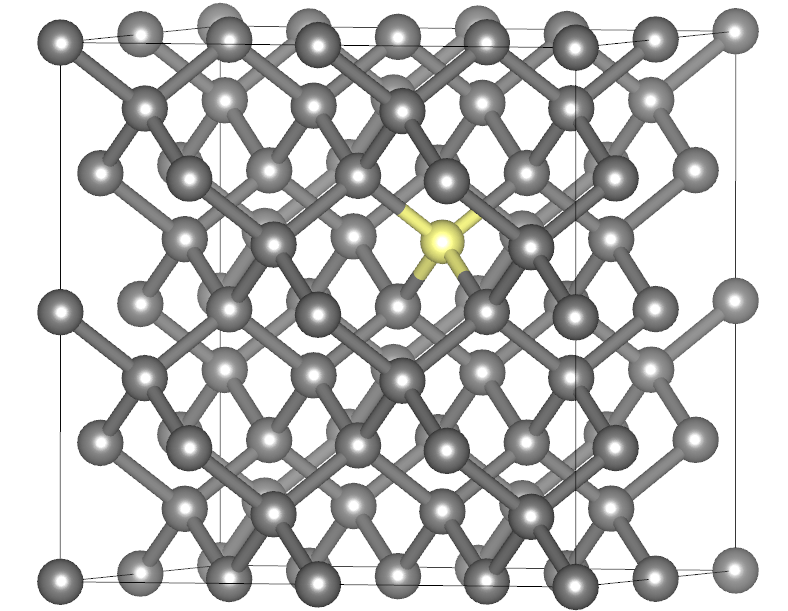
\includegraphics[width=0.5\textwidth]{figures/Diamond_CCenter_SubN.png}
    \caption{The C or P1 Center (N\textsubscript{s}) nitrogen-related defect in diamond. Nitrogen atoms are shown in yellow and carbon atoms are shown in gray.}
    \label{fig:P1Center}
\end{figure}
    
\begin{figure}
    \centering
    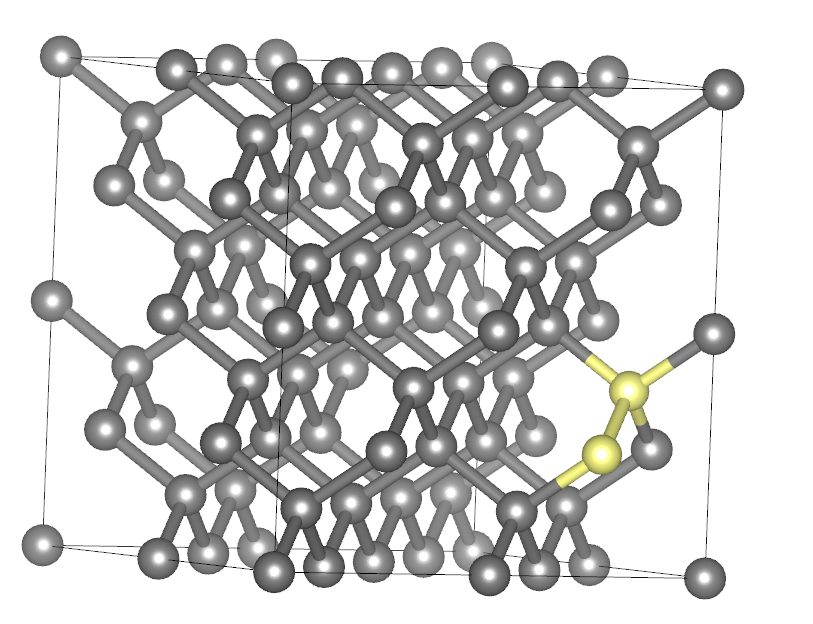
\includegraphics[width=0.5\textwidth]{figures/Diamond_ACenter_2N.png}
    \caption{A center (N\textsubscript{2}) nitrogen-related defect in diamond. Nitrogen atoms are shown in yellow and carbon atoms are shown in gray.}
    \label{fig:Acenter}       
\end{figure}
    
\begin{figure}
    \centering   
    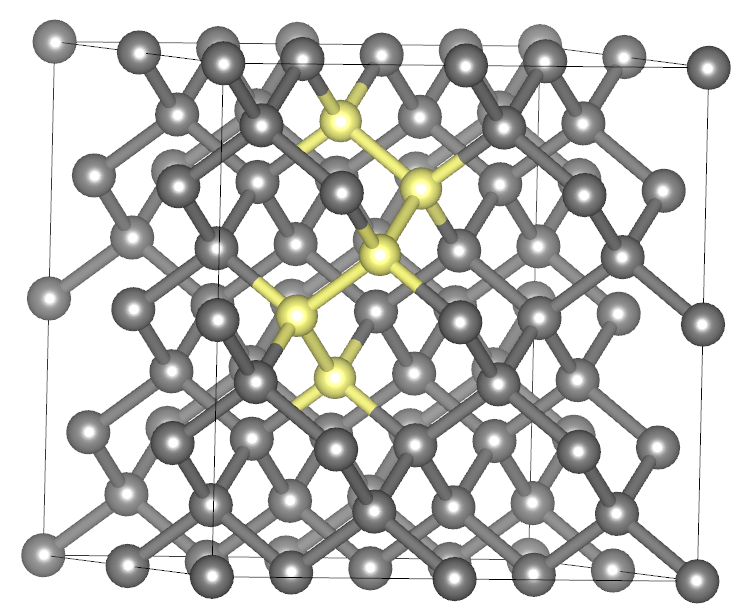
\includegraphics[width=0.5\textwidth]{figures/Diamond_N_Platelet_5N_Rectangular.png}
    \caption{Nitrogen Platelet (N\textsubscript{platelet}) nitrogen-related defect in diamond. Nitrogen atoms are shown in yellow and carbon atoms are shown in gray.} 
    \label{fig:NPlatelet}
\end{figure}
    
\begin{figure}
    \centering
    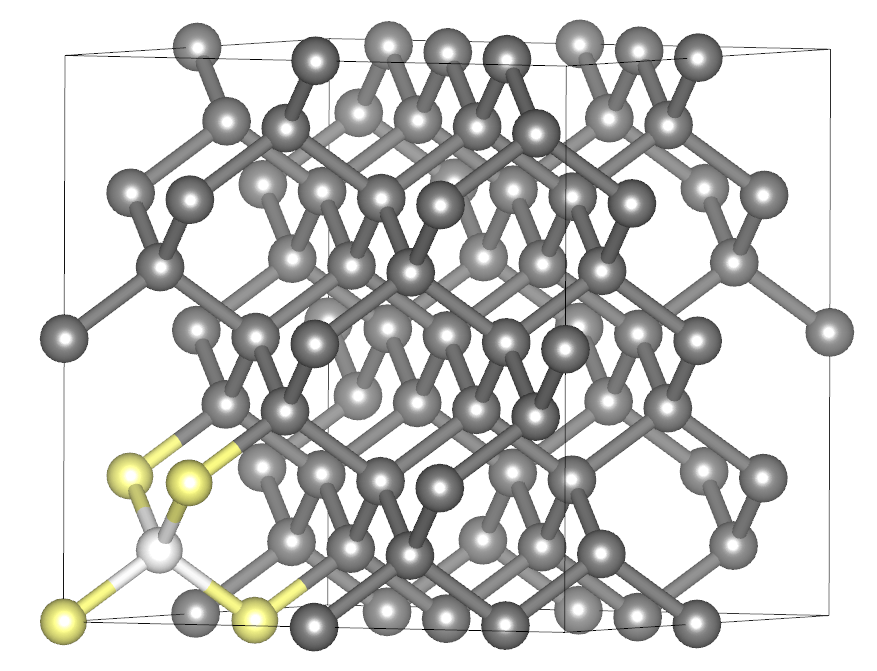
\includegraphics[width=0.5\textwidth]{figures/Diamond_BCenter_N4V.png}
    \caption{B or P2 center (N\textsubscript{4}V) nitrogen-related defect in diamond. Nitrogen atoms are shown in yellow, carbon atoms are shown in gray, vacancies are represented by white atoms.}
    \label{fig:Bcenter}
\end{figure}

Because the FTIR measurements in this work were taken at room temperature, the absorption peaks exhibit thermal broadening. This makes it difficult to resolve individual absorption peaks across the 1050 cm\textsuperscript{-1} to 1400 cm\textsuperscript{-1} region where a high density of nitrogen-related defects absorption occurs. A peak deconvolution method was developed to resolve individual absorption peaks for specific nitrogen related defects. Absorption peaks are deconvoluted by fitting the region of interest (1050 cm\textsuperscript{-1} to 1400 cm\textsuperscript{-1}) with seven relevant, nitrogen-related peaks. The fit can be compared to the actual absorption spectrum. If a strong fit is observed, individual absorption peak intensities and location have been accurately resolved and can be used to calculate the concentration of specific nitrogen related defects. An exemplary results of this method is shown in Figure \ref{fig:FTIRfitFTD2417a}.

\begin{figure}
    \centering
    \includesvg[width=\textwidth]{figures/FTD24_17a_ROI_Fit.svg}
    \caption{Seven Gaussian peaks corresponding to nitrogen related defects fit to the FTIR absorbance spectrum of FTD24\_17a. The fit has strong agreement with the data as an R\textsuperscript{2} value of 0.9986 was calculated.}
    \label{fig:FTIRfitFTD2417a}
\end{figure}

Eight single crystal diamond sample were used to develop this method. Deposition details for the samples can be found in Chapter \ref{chPressureOffcut} Section \ref{pressureOffcutRedo}. Transmission spectra were taken on the starting substrate as well as the sample after deposition (substrate+grown film). Three transmission spectra were averaged per sample. The starting substrate spectrum was subtracted from the spectrum of sample after deposition and divided by grown film thickness to find IR absorption coefficient for just the grown film. Then, seven Gaussian functions corresponding to nitrogen-related defect absorption at 1130 cm\textsuperscript{-1}, 1180 cm\textsuperscript{-1}, 1215 cm\textsuperscript{-1}, 1280 cm\textsuperscript{-1}, 1332 cm\textsuperscript{-1}, 1344 cm\textsuperscript{-1}, and 1360 cm\textsuperscript{-1} were fit to the 1050 cm\textsuperscript{-1} to 1400 cm\textsuperscript{-1} region. The peaks were allowed to shift from the starting point by up to $\pm$ 3 cm\textsuperscript{-1} to accommodate for strain shift while keeping the physical relevance. Some defects absorb at more than one wavenumber within this region. The different absorption correspond to different vibration modes of the defect. Two intensity constraints, Equation \ref{P1ConstraintEqn} and Equation \ref{plateletConstraintEqn}, were made to fix the ratio of vibrational mode absorption peaks for the P1 center and platelets thereby constraining the model and minimize overfitting \cite{Lawson1998OnDiamond, Woods1986PlateletsDiamonds}.

\begin{equation}
    \mu_{1344}=0.57\mu_{1130}
    \label{P1ConstraintEqn}
\end{equation}

\begin{equation}
    \mu_{1360}=0.365\mu_{1280}.
    \label{plateletConstraintEqn}
\end{equation}

After a fit is found, the more accurately defined peak parameters can be extracted from the model. Then, the concentration of N\textsubscript{S}\textsuperscript{0} and nitrogen platelets can be calculated using Equation \ref{subNconcEq} and Equation \ref{aggNConcEq}, respectively. The total nitrogen concentration in diamond can be determined using Equation \ref{totalNConcEq}.  

\begin{equation}
    [N_s^0]=A_{1130}K_{S2}
    \label{subNconcEq}
\end{equation}
\begin{equation}
    [N_{platelet}]={A_{1280}}{K_{A2}}
    \label{aggNConcEq}
\end{equation}
\begin{equation}
    [N_{total}]=[N_{platelet}]+[N_S^0]
    \label{totalNConcEq}
\end{equation}

The proportionality coefficients, K\textsubscript{S2} and K\textsubscript{A2}, were found by fitting a weighted sum of the peak area for N\textsubscript{S}\textsuperscript{0} and nitrogen platelets to spin concentration. Spin concentration could be quantitatively determined through EPR by establishing a calibration curve. The calibration curve, Figure \ref{fig:BDPAcalibration}, was generated using a stable organic radical, $\alpha$,$\gamma$-bisdiphenylene-$\beta$-phenylallyl (BDPA), diluted in a diamagnetic potassium bromide (KBr)\cite{Mandal2020OnRadicals}. The known concentration of unpaired electrons in each BDPA dilution is correlated to the double integral of the EPR signal. The double integral of an EPR signal in diamond substrates can, then, be converted to spin concentration.

\begin{figure}
    \centering
    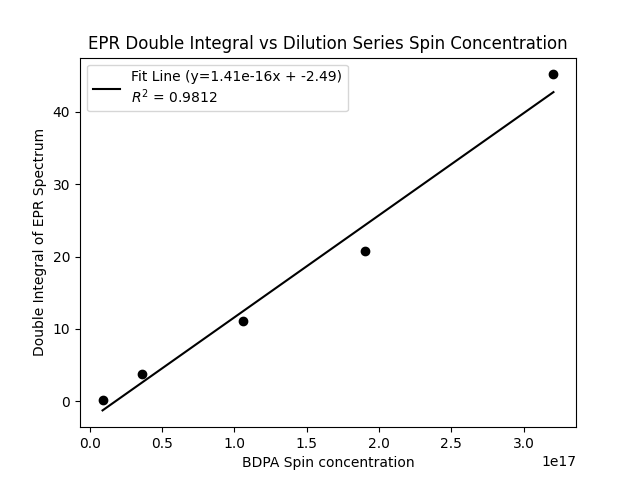
\includegraphics[width=\linewidth]{figures/EPRCalibrationCurveStandardLinearFitExcludesUndiluted.png}
    \caption{Correlation of EPR double integral with BDPA dilution series spin count. This fit excludes the undiluted sample.}
    \label{fig:BDPAcalibration}
\end{figure}

\section{Validation of Fourier Infrared Transform Spectroscopy Method via Electron Paramagnetic Resonance}
\indent

EPR was used to validated the improved FTIR method for determining nitrogen concentration described in Section \ref{improvedFTIRMethod}. EPR spectra were taken on eight diamond samples. A total spin concentration was calculated using the BDPA calibration curve. This spin value was plotted against a weighted sum of the 1130 cm\textsuperscript{-1} and 1280 cm\textsuperscript{-1} peak areas measured using the new FTIR as shown in Figure \ref{fig:EPRvalidationFTIR}. In Equation \ref{subNconcEq} and Equation \ref{aggNConcEq}, the calibration coefficients K\textsubscript{S2} and K\textsubscript{A2} are the weighting of the respective FTIR peak. This method gives calibration coefficients of K\textsubscript{S2} = 49.54 ppm/cm\textsuperscript{-2} and K\textsubscript{A2} = 51.84 ppm/cm\textsuperscript{-2} for nitrogen-rich diamond.

\begin{figure}
    \centering
    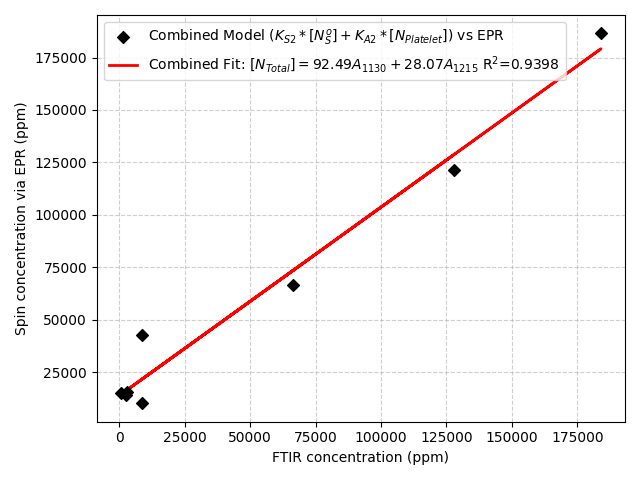
\includegraphics[width=0.8\linewidth]{figures/Weighted_Average_Fit_Using_Area_All_FixPeakRatio.png}
    \caption{EPR double integral of diamond samples against weighted average of 1130 cm\textsuperscript{-1}and 1280 cm\textsuperscript{-1} FTIR peak area. The weighted average of FTIR peak area corresponds to the total nitrogen concentration.}
    \label{fig:EPRvalidationFTIR}
\end{figure}

The total nitrogen concentration as determined using the improved FTIR method exhibits strong positive correlation with spin concentration via EPR, most notably at high concentrations of nitrogen. 

\section{Improved Detection of High Concentrations of Substitutional Nitrogen}
\indent

This newly developed method for determining substitutional nitrogen concentration in diamond was compared to the previously established method. Nitrogen concentration was calculated using both methods and compared to spin concentration as determined with EPR. The results are shown in Figure \ref{fig:improvedFTIRvsKiflawi}. At moderate concentration of nitrogen, the methods are comparable. At high concentrations of nitrogen, however, the newly developed method outperforms the Kiflawi method.

\begin{figure}
    \centering
    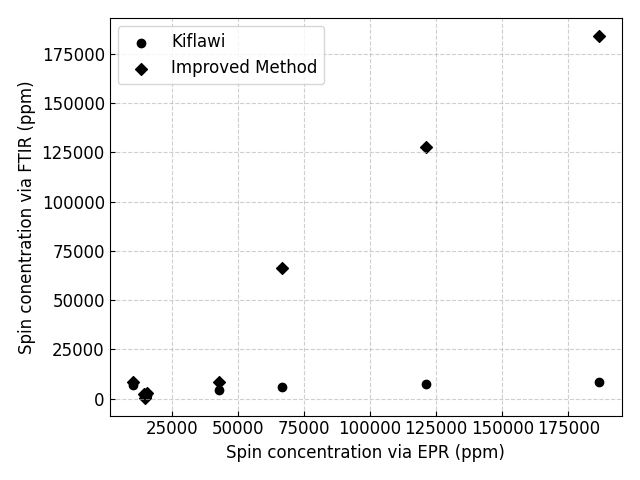
\includegraphics[width=\linewidth]{figures/Kiflawi_Model_vs_Improved_Model.png}
    \caption{Comparison of the improved method of this work to Kiflwali Method.}
    \label{fig:improvedFTIRvsKiflawi}
\end{figure}

The FTIR method to determine nitrogen concentration in nitrogen-rich diamond using absorption peak area found through peak deconvolution of and FTIR spectrum demonstrated improved accuracy of nitrogen concentration when compared to the Kiflawi method.